%!TEX root = dolgozat.tex
%%%%%%%%%%%%%%%%%%%%%%%%%%%%%%%%%%%%%%%%%%%%%%%%%%%%%%%%%%%%%%%%%%%%%%%
\chapter{Technical details}\label{ch:IMPLEMENTATION}

\section{Architecture}

E-me follows a commonly used N-tier architecture with three main parts: data, application (backend) and presentation (frontend) layers.
Each of these tiers can be broken down into layers that are defined by their responsibilities within the application.
This tier-based architectural approach adds modularity to the application which results in a low cost of change when compared to a single-tier structure.

\begin{figure}[h]
	\centering
	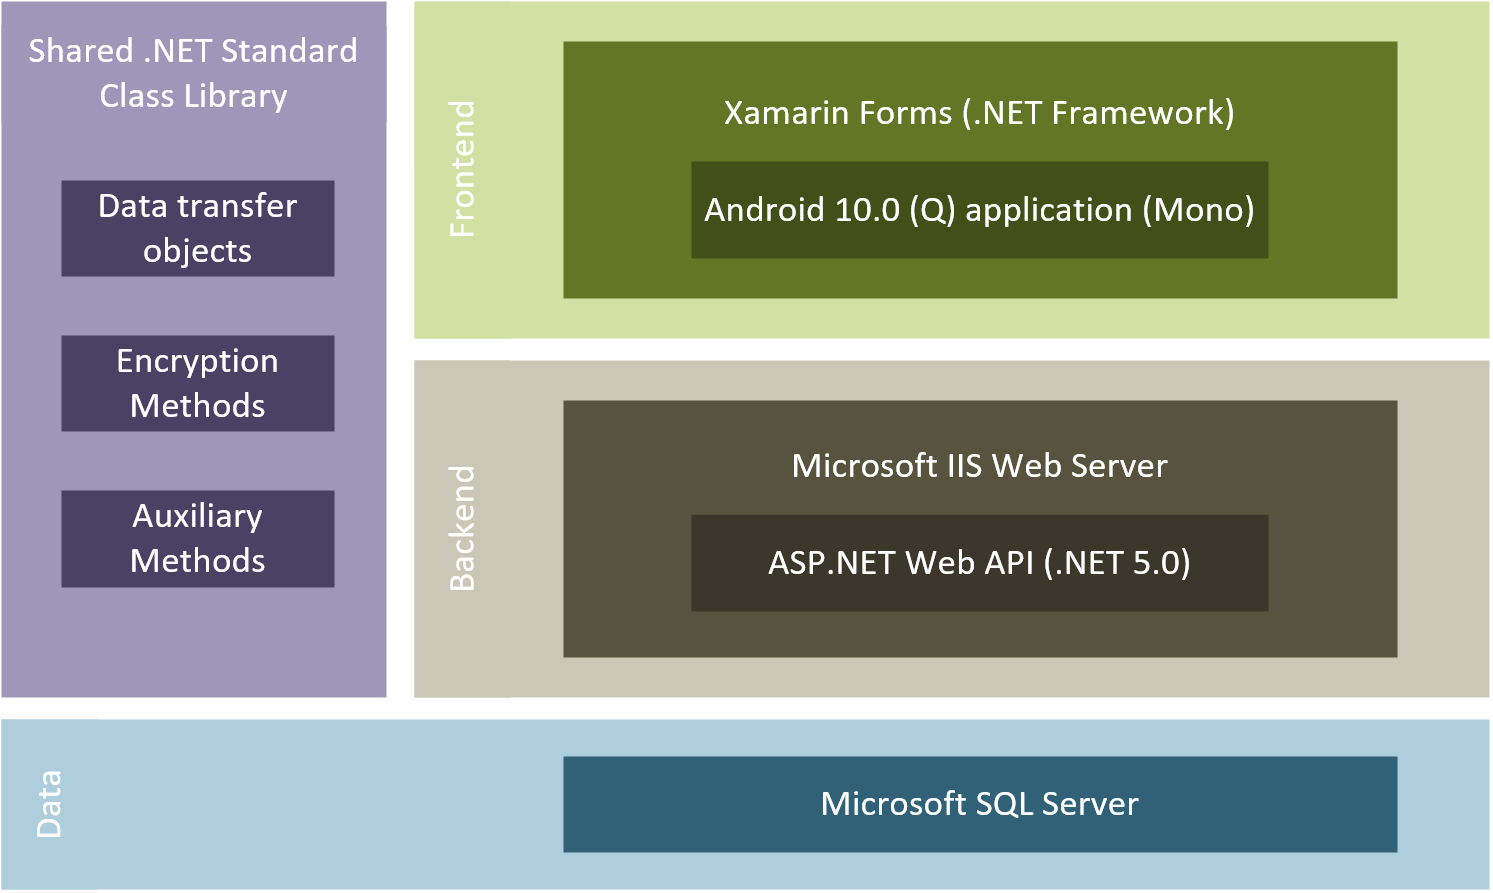
\includegraphics[scale=0.40]{general-architecture.png}
	\caption{General architecture}
\end{figure}

Along with the low cost of change, the independence of the layers allows for efficient future expansion of 
the application by means of multiple frontend platforms (ex. web applications, desktop applications), cloud storage/services and additional
Web API's that can easily be integrated into the existing application.
This, combined with the high compatibility of the .NET 5.0, provides a high level of scalability and maintainability for the application.

The application and presentation layers share a common class library that contains communication-related models and auxiliary methods.
This library allows both layers to benefit from the cross-platform nature of .NET 5.0, speeding up the process of development and
ensuring there are no discrepancies betweeen the layers in terms of encryption and communication.

\subsection{Application layer / Backend}

The architecture of the application layer has a similar design approach to the general architecture.
Consisting of 4 layers, the backend follows the single-responsibility principle in it's core.
Because of it's vertical structure, each layer is dependent on one single layer that is directly below it, providing a high level
of maintainability.

\begin{figure}[H]
	\centering
	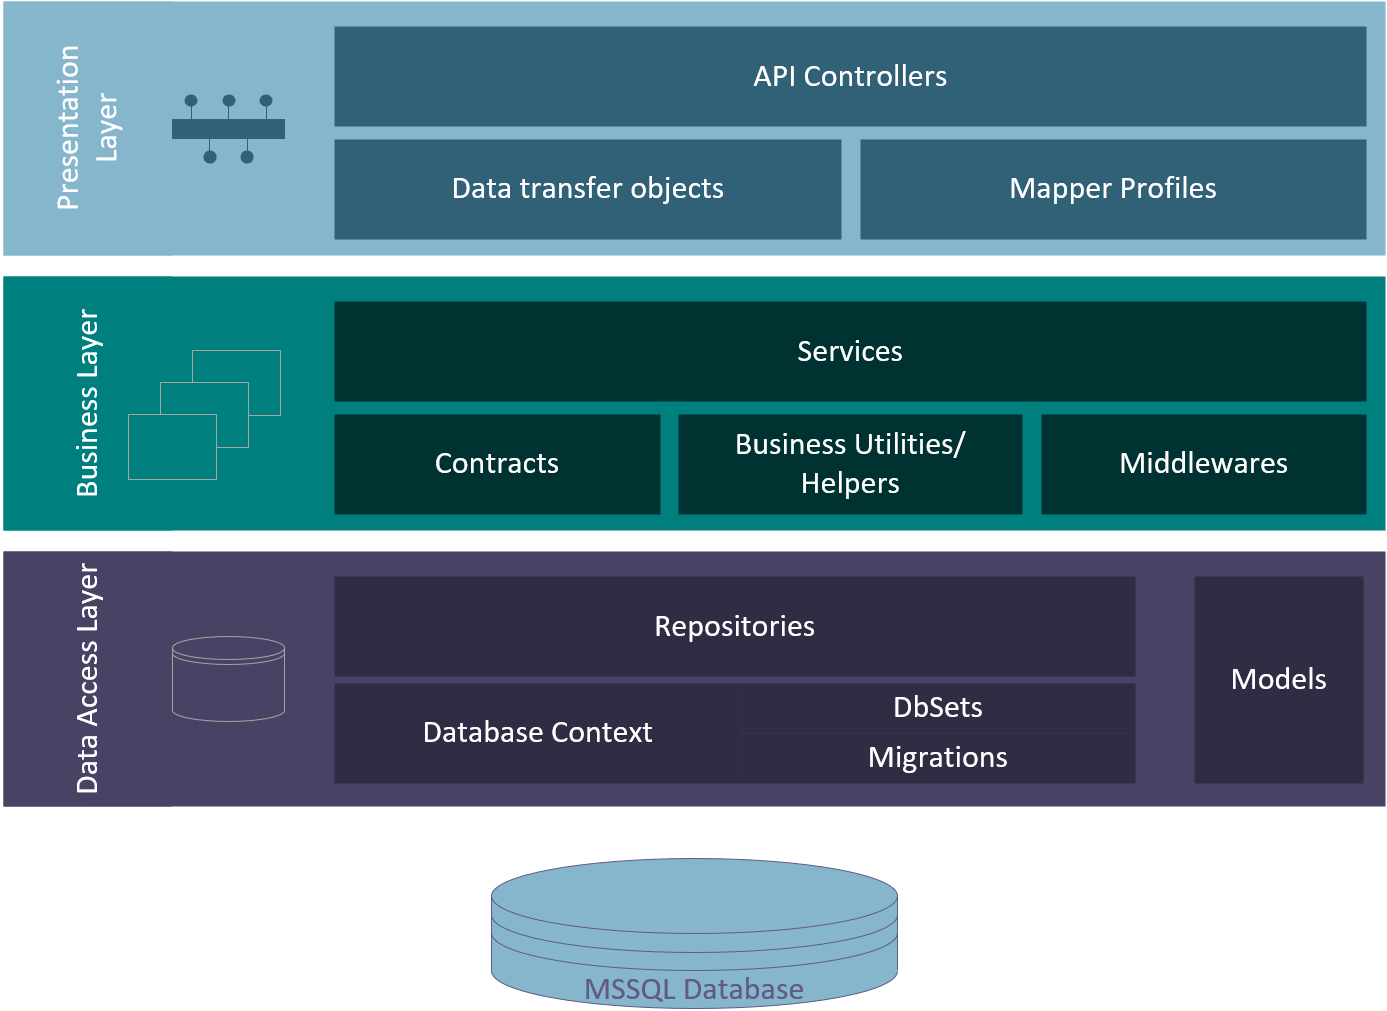
\includegraphics[scale=0.40]{backend-architecture.png}
	\caption{Backend architecture}
\end{figure}

Due to this abstract layout, each layer can independently be replaced or updated. 
This aspect enables the utilization of external and/or third-party services and components without damaging the integrity of the application.

The API structure of the presentation layer allows for a wide variety of applications or even services in which the backend can be used: desktop applications,
WPF, web servers and more. This characteristic has major role in preserving the flexibility of the application layer.

Another component being responsible for the independece and reusability of the backend is the Data Access Layer. 
The role of this layer is to provide the data requested by the Business Layer. 
By reason of abstraction, this layer is independent of the technology of the data source. 
This enables the utilization of a wide range of data sources, including relational (SQL) and non-relational (NoSQL) databases, cloud services and/or APIs.

\subsubsection{Entity relations in the database layer}

\begin{figure}[H]
	\centering
	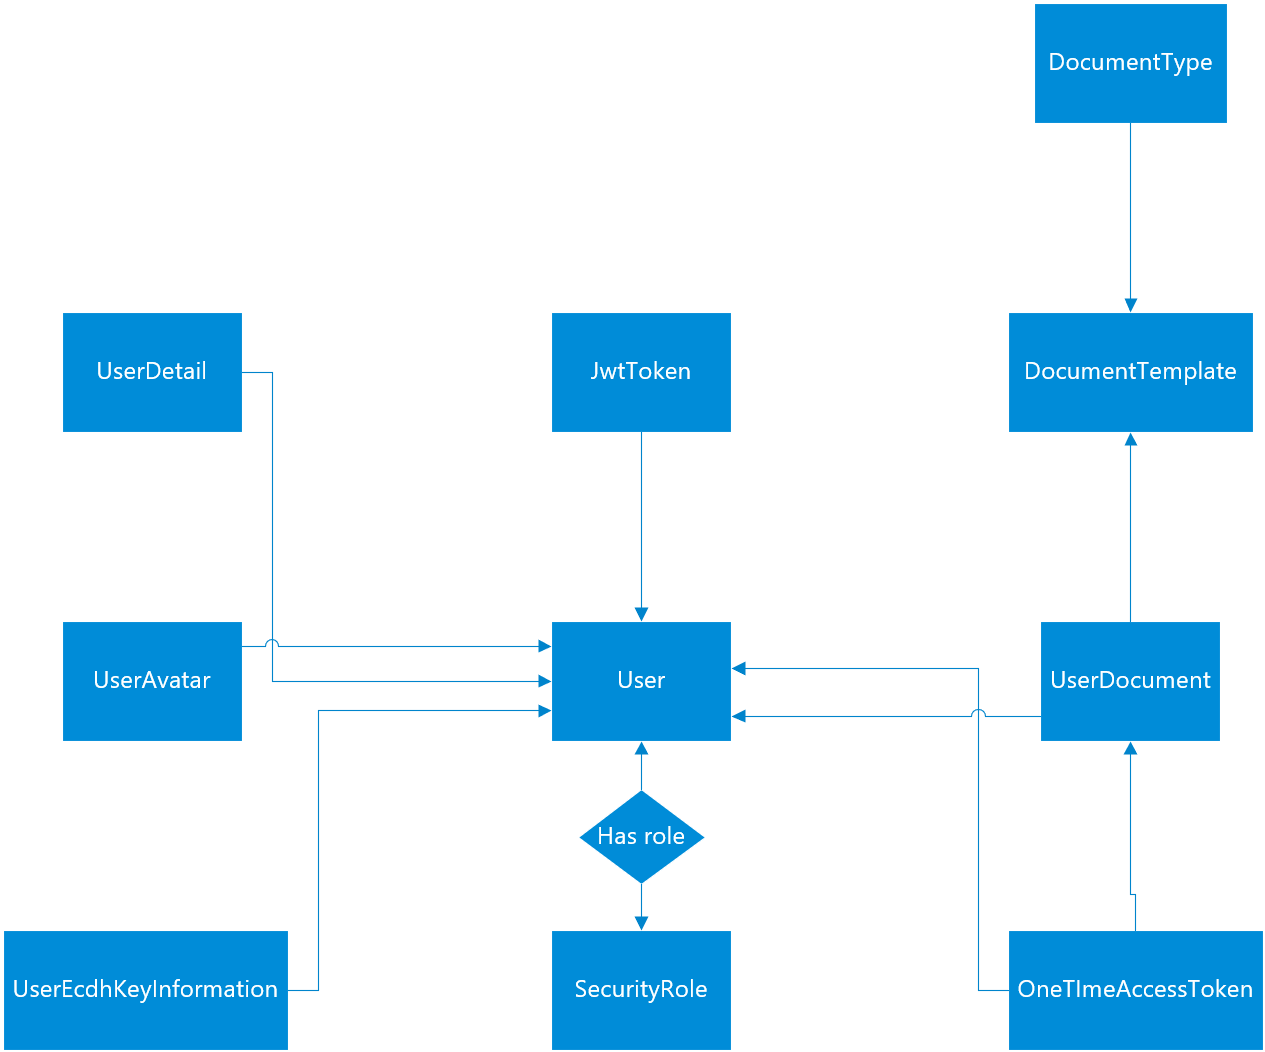
\includegraphics[scale=0.37]{entity-relationship-diagram.png}
	\caption{Entity-relationship diagram}
\end{figure}

\subsection{Presentation layer / Frontend}

The frontend of the application consists of three major layers that separate the user interface from the business logic and the data sources.
This separation allows for easy horizontal expansion and quick feature development.

The Presentation or UI Layer contains the visuals of the application which are separated into independent pages, however it is also responsible for receiving
user events and connecting them with the underlying services.
Each page contains it's own event listeners and separate View Model that is responsible for making use of the Business Layer,
which has a similar structure and role to the backend's Business Layer: data processing and calculations.

The main components of the Data Layer are Data Stores.
These stores are functionally similar to the repositories found in the Backend of the application, although here the data is retrieved using the endpoints
of the backend.

\begin{figure}[H]
	\centering
	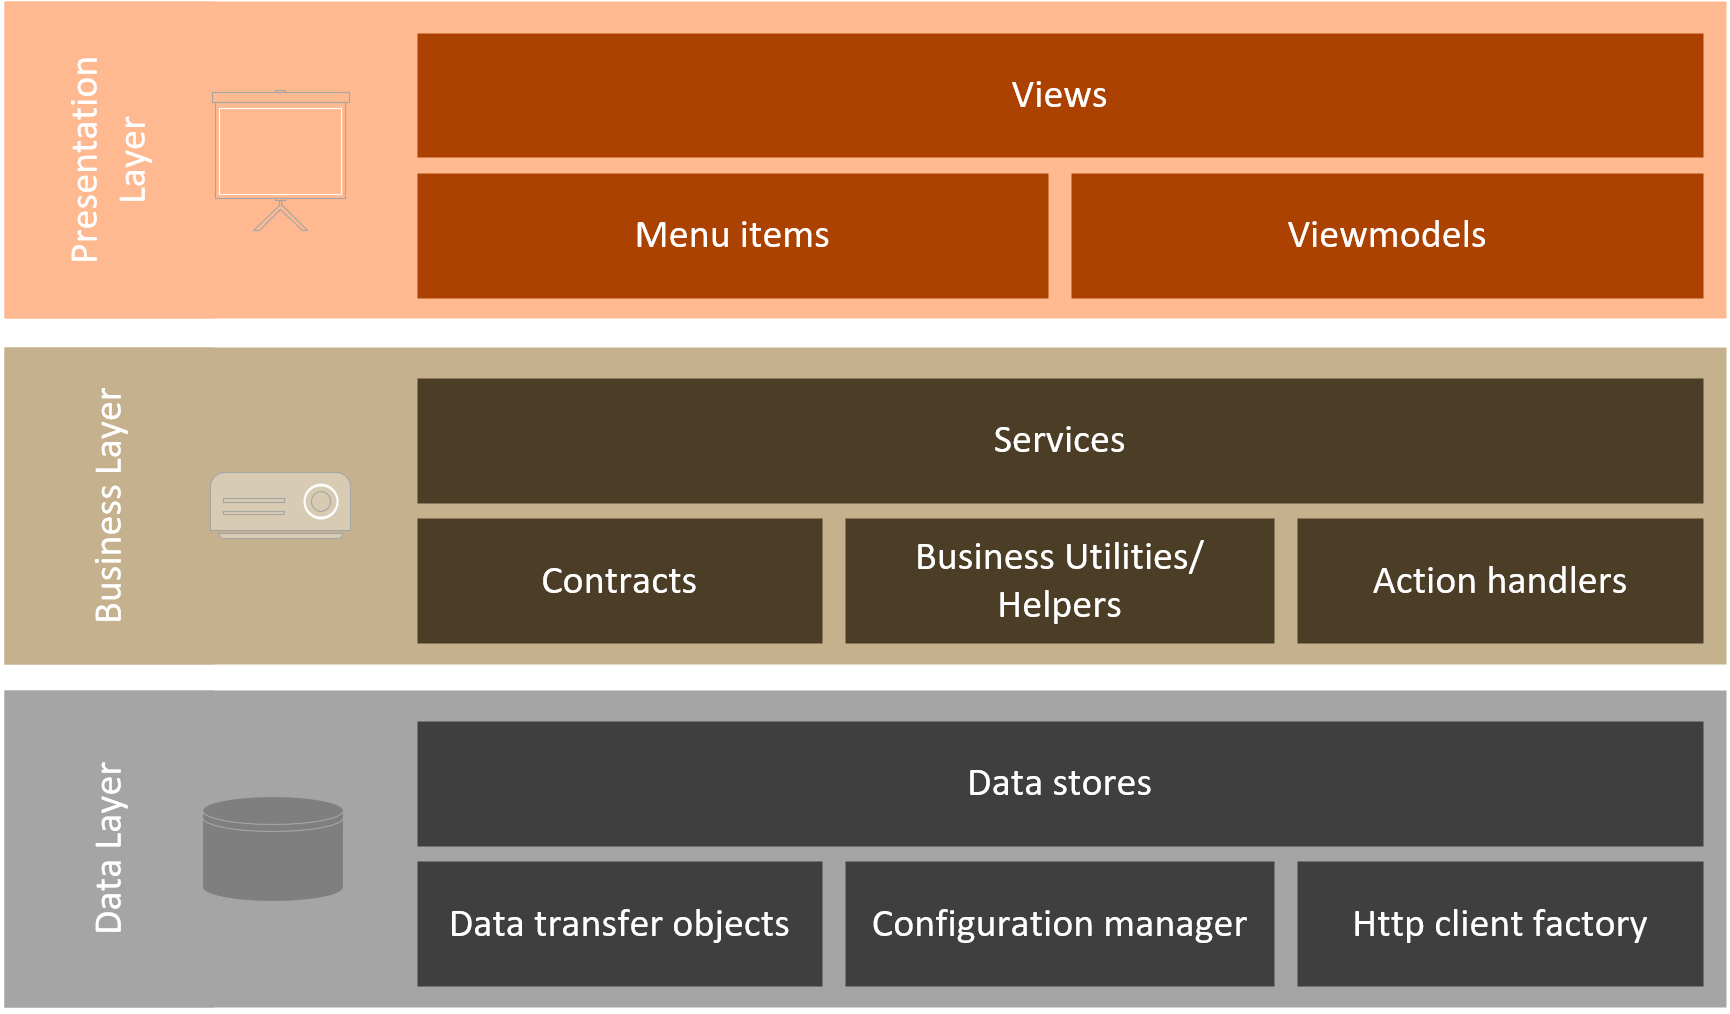
\includegraphics[scale=0.32]{frontend-architecture.png}
	\caption{Frontend architecture}
\end{figure}


%%%%%%%%%%%%%%%%%%%%%%%%%%%%%%%%%%%%%%%%%%%%%%%%%%%%%%%%%%%%%%%%%%%%%%%
\section{Technologies}

E-me makes great use of the cross-platform nature of .NET, meaning both the frontend and the backend of the application are implemented using the same
programming language: C\# 9.
The flexibility that is provided by the language and the wide variety of frameworks that make use of it allows for a cleaner codebase and a simpler
project structure when compared to a multilingual application design.

\subsection{Backend}

In terms of frameworks, the backend relies on .NET 5.0. Being the next major release of .NET Core following 3.1, this open-source cross-platform
software framework unifies a wide variety of frameworks .NET has to offer, including Windows Forms, ASP.NET Core, Azure and more.
This unification made the framework a perfect candidate for the backend of an application like E-me, since it can be used on a wide variety of
platforms and ensures long-term support.

E-me uses Internet Information Services (Microsoft IIS), which is an extensible web server software, as it's backend server.
It allows the application to communicate through HTTPS and provides it's separate development-time SSL certificate in order to secure the transport
layer. With the \emph{Development-time IIS support} feature, the web server allows \emph{hot reloading}, which speeds up the development and debugging
processes.

The main constituent of the backend itself is the ASP.NET Core web framework.
Using it's built-in IoC, this framework allows for a high level of abstraction in order to build well-structured enterprise level applications
using dependency injection.
This framework is responsible for registering and configuring any other dependencies that may appear in the application backend.

Alongside with ASP.NET Core, one of the main components of the backend is the Entity Framework Core, which is the base of the 
\emph{Data Access Layer}.
In terms of building and maintaining the data access layer, E-me uses the code-first approach through \emph{EF Migrations}.
This approach provides flexibility in case of a potential database change and/or creation, but more importantly it allows 
the entire structure of the entities to be managed based on the models and datasets present in the code.

E-me heavily relies on encryption and security, which demands the utilization of advanced cryptographic libraries.
For this purpose, the application uses the \emph{Windows CNG (Cryptographic Next Generation) API}, which
enables exchanging documents and other data in a secure environment.
In terms of cryptography, this API provides a full implementation of the \emph{Elliptic-curve Diffie-Hellman} key agreement protocol,
alongside with many other cryptographic protocols and algorithms such as RSA, AES (Advanced Encryption Standard) or DSA (Digital Signature Algorithm)
and hash functions like SHA-2 or MD5.

The documents handled by the application are created and managed by the \emph{Telerik Document Processing Core} framework, which
provides flexibility and efficiency in terms of document management. 
It enables processing the most commonly used text, PDF and spreadsheet file formats, allowing the application
to create, import and export documents without relying on other external dependencies.

\subsection{Frontend}

Being a .NET-based application, E-me uses Microsoft's open-source mobile UI framework, \emph{Xamarin Forms} as a base for it's frontend.
This library allows developing native mobile applications on multiple platforms, such as iOS, Android or UWP using \emph{.NET Standard}. 
The multi-platform capability allows for a shared codebase and logic across all applications, which speed up the development process immensely.
Xamarin uses an XML-based interface designer in order to create the visuals for the application.
Alongside with the commonly used Xamarin UI components, E-me uses the \emph{Telerik UI for Xamarin, GoogleVision API and Syncfusion} UI
libraries for additional components and controls in it's user interface.



Although the frameworks used by the different layers of the application vary, these can have a shared codebase in the form
of a \emph{.NET Standard class library}, which can be used by both the backend and the frontend, allowing for closely integrated layers.

\section{Implementation}

Being cross-platform and having a wide range of possibilities in terms of future expansion and upgrades, E-me focuses heavily on scalability and maintainability.
In order to achieve these characteristics, multiple factors have to be considered during development, such as project structure, dependencies and code reusability.
For this purpose, both the backend and the frontend of the application relies on \emph{Dependency Injection}.
This technique allows for a service-based structure within the application and it is an elegant way of implementing loosely coupled classes.

\subsection{Backend}

The backend of E-me is separated into 5 projects that are defined by their role within the application.
These projects are targeting the \emph{.NET 5.0} framework, one exception being the \emph{Shared} project, which is used as the common
codebase for the backend and the frontend.
The majority of the projects are \emph{Class Libraries}, which are collections of pre-coded object-oriented templates and classes. 
These libraries revolve around the main entry-point of the application, the \emph{MVC project}.

\subsubsection{The MVC project}

As the main entry-point of the application backend, this project is responsible for configuring and registering all dependencies and services
E-me requires and utilizes.
This configuration of the \emph{IoC (inversion of control)} and the registration of dependencies take place in the \emph{Startup} class.
This class is registered to the \emph{Host Builder} as soon as the application starts.

\begin{lstlisting}
  public static IHostBuilder CreateHostBuilder(string[] args)
  {
	return Host.CreateDefaultBuilder(args)
		.ConfigureWebHostDefaults(webBuilder =>
		{
			webBuilder.UseStartup<Startup>();
		});
  }
\end{lstlisting}

This project defines the \emph{API Controllers} which are representing the endpoints of the backend.
These controllers are the connection points through which the backend is able to communicate with other layers of the application.

One of the most important of these controllers is the \emph{AuthController}, which is responsible for 
registering, authenticating and de-authenticating the users of the application.
This is the only controller that can be accessed by an unauthenticated user, since the rest of them handle more 
sensitive data.

\begin{figure}[H]
	\centering
	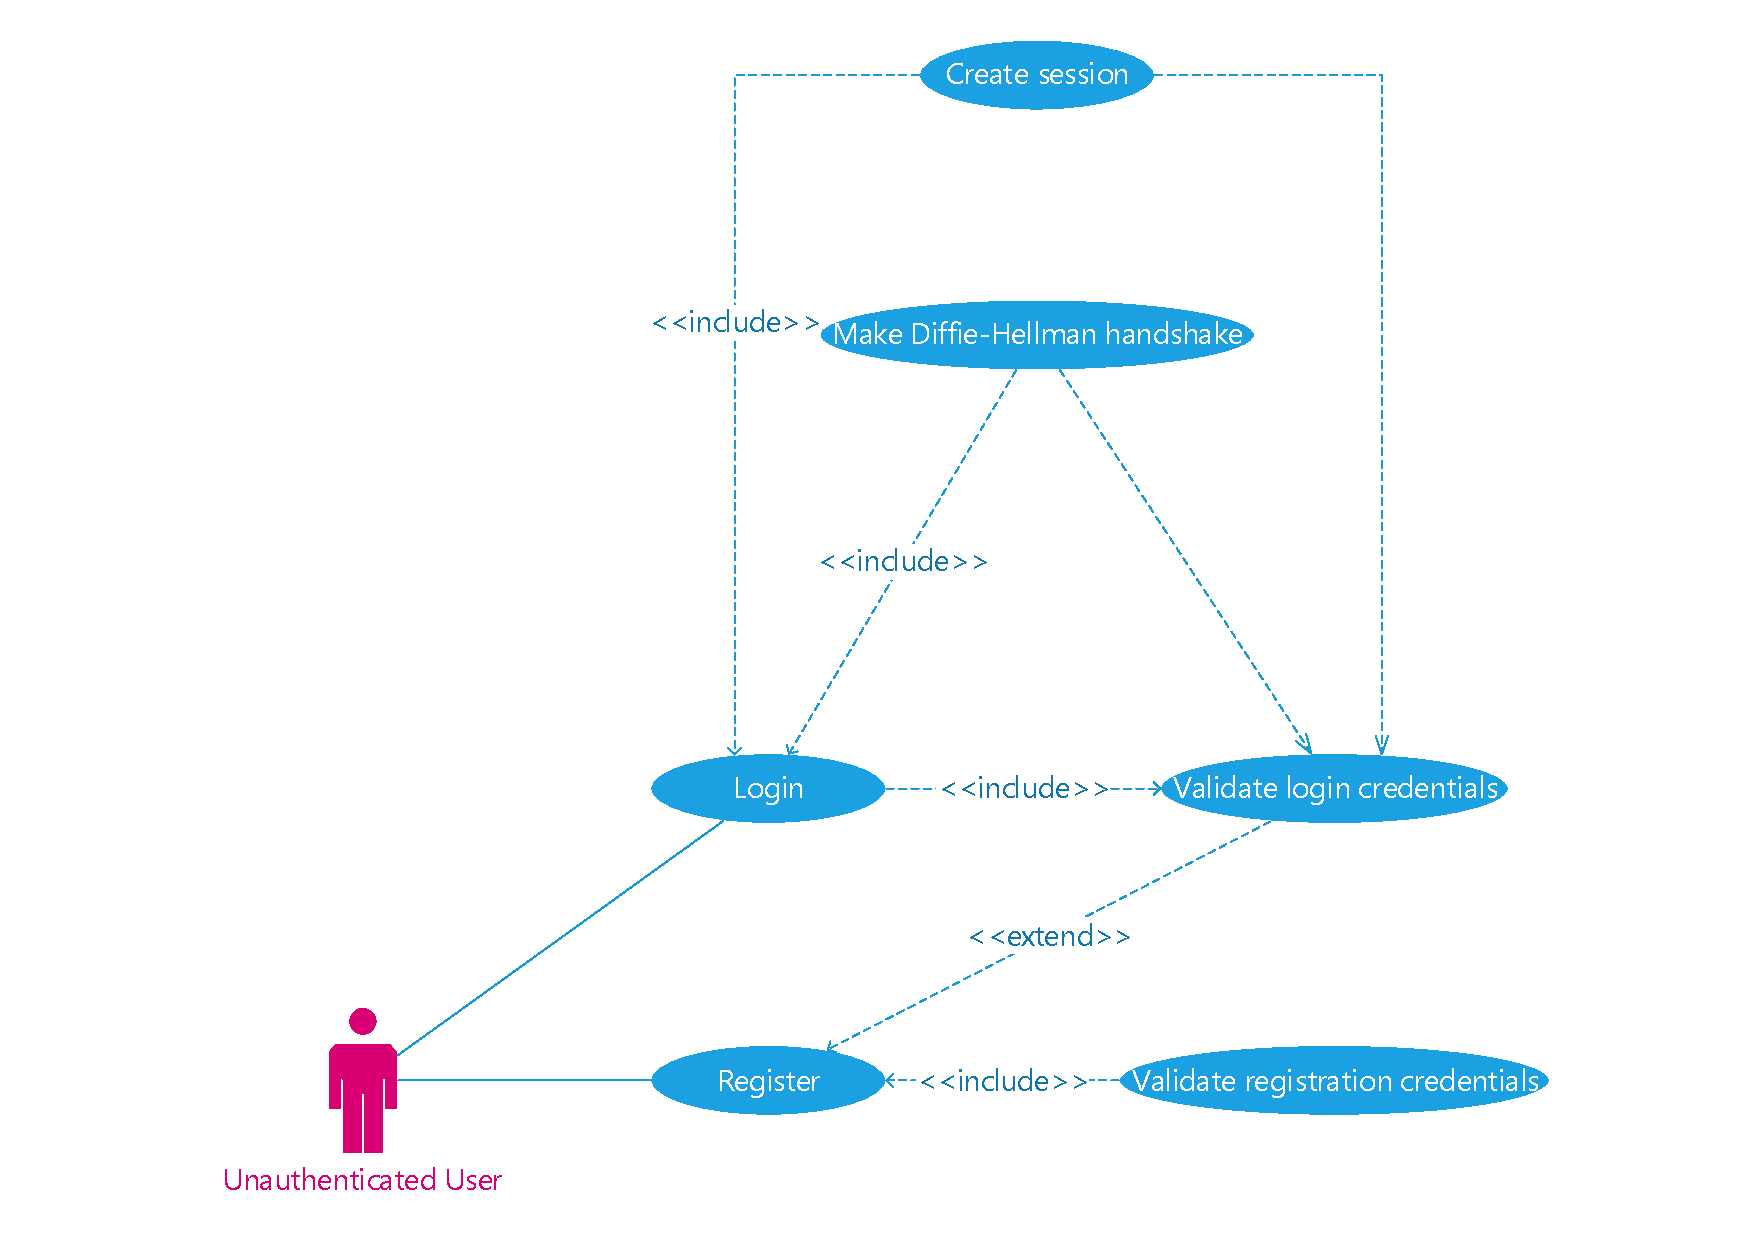
\includegraphics[scale=0.50]{use-case-diagram-unauth}
	\caption{Use-case diagram (unauthenticated user)}
\end{figure}

Once a user is authenticated, they are able to access the rest of the endpoints.
A controller's or and endpoint's 

\begin{figure}[H]
	\centering
	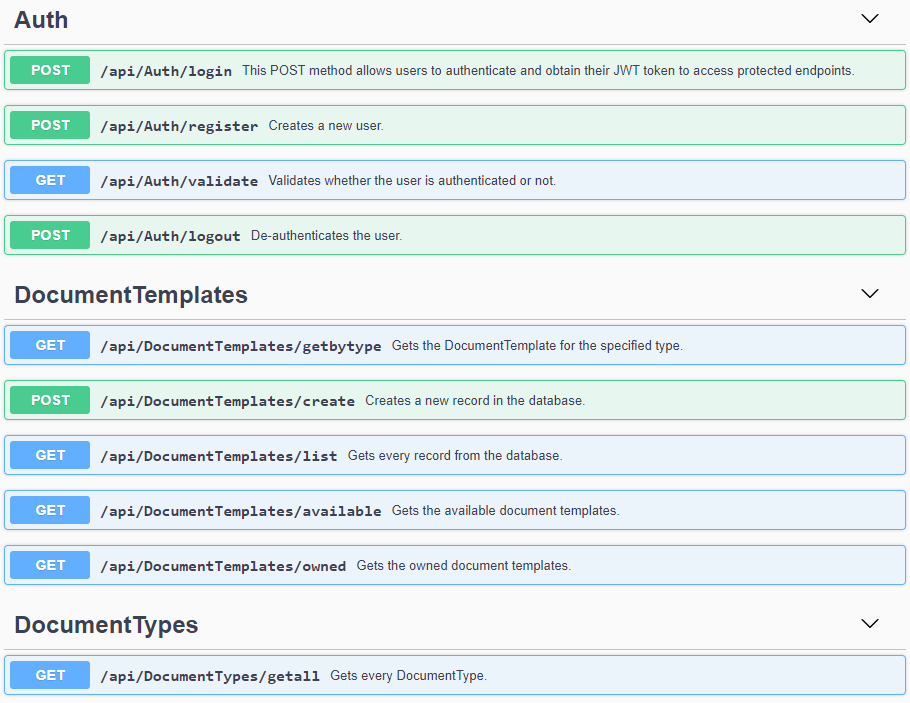
\includegraphics[scale=0.65]{swagger1.png}
	\caption{API endpoints (1)}
\end{figure}

\begin{figure}[H]
	\centering
	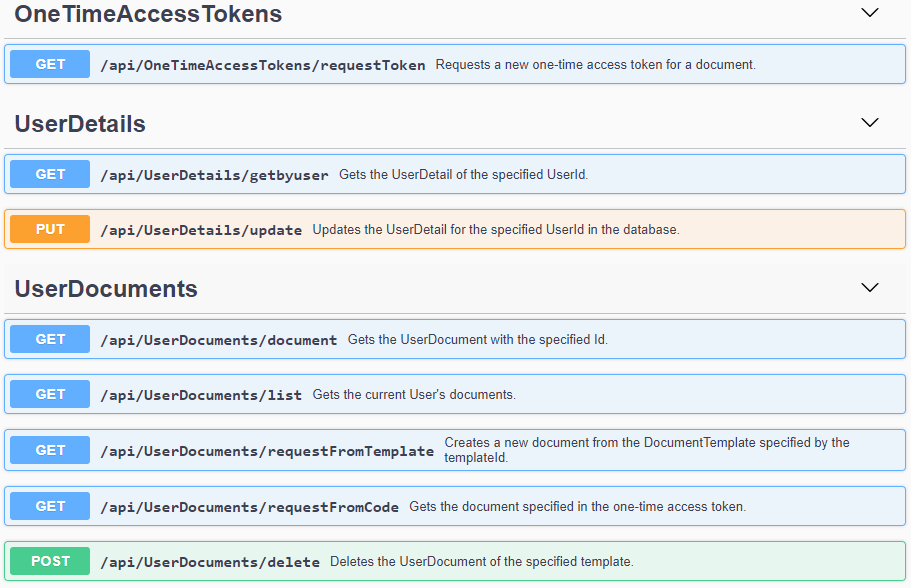
\includegraphics[scale=0.65]{swagger2.png}
	\caption{API endpoints (2)}
\end{figure}



\begin{figure}[H]
	\centering
	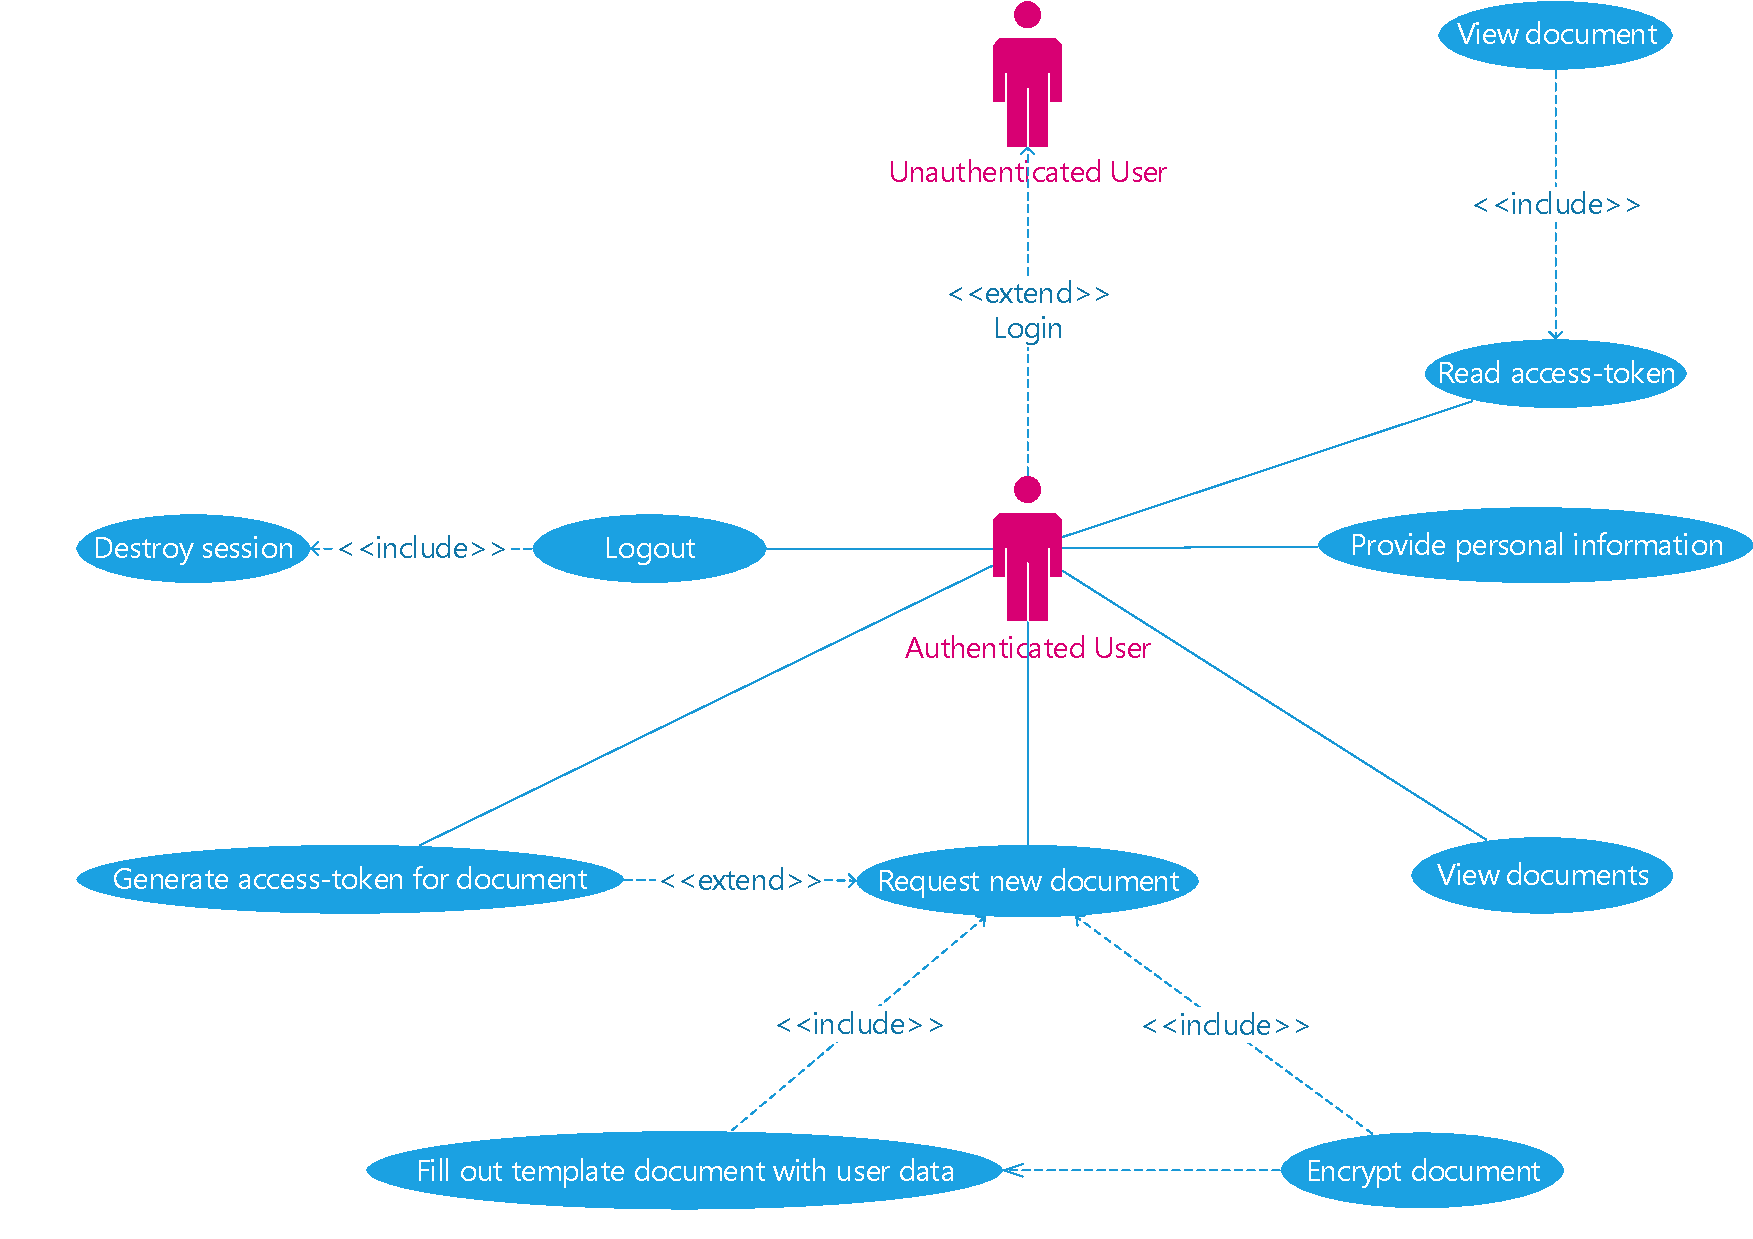
\includegraphics[scale=0.50]{use-case-diagram}
	\caption{Use-case diagram (authenticated user)}
\end{figure}

\section{Security}

As a document-handling application, E-me relies heavily on secure communication, data storage and encryption.
In order to achieve the required level of protection, the application uses a handful of libraries that target various layers within the backend and the frontend.

\subsection{Data-layer security}

First and foremost, E-me utilizes \emph{Entity Framework Core Data Encryption}, which is a plugin for the above mentioned \emph{Entity Framework Core},
 to add support of encrypted fields using built-in or custom encryption providers.
This library ensures the protected storage of the data via encryption.
This way the data stored in the database cannot be interpreted by other parties, not even in a case of a security breach or database failure.
In the case of E-me, a built-in encryption provider is used which enables \emph{AES-256} encryption configured with a CBC (cipher-block chaining) cipher.
The algorithm uses a secret key stored in the configuration of the application.

\begin{lstlisting}
  private AesProvider CreateAesProvider()
  {
	var key = Encoding.ASCII.GetBytes(_authSettings.SecretKey);
	var provider = new AesProvider(key, CipherMode.CBC,	 PaddingMode.Zeros);
	return provider;
  }
\end{lstlisting}

The data encryption library allows for independent protection of model attributes, providing flexibility for the developers in selecting sensitive fields
that require encryption. This selection can greatly reduce the time consumption of the encryption and is preformed via the \emph{Encrypted} field attribute:

\begin{lstlisting}
  [Encrypted]
  public string FullName { get; set; }
\end{lstlisting}

\subsection{End-to-end encryption (E2EE)}

The second layer of security is located in the \emph{Business Layer} of the application backend.
One of the main features of E-me is the end-to-end encrypted (E2EE) document transfer which is achieved by this second layer.
In order to successfully perform an encryption on the backend followed by a decryption on the frontend, the two sides must complete a secure key exchange beforehand.
This exchange occurs upon a user's successful login to the system.

Upon receiving the user's credentials, a key pair (private and public keys) is generated on the frontend of the application.
The key generation and derivation takes place in the \emph{EcdhKeyStore} class which uses a password-based key derivation functon (\emph{PBKDF2}) with a \emph{SHA512} hash function
as the private key generator and \emph{X25519 Elliptic Curve Diffie-Hellman} to derive a public key from the generated private key.

\begin{lstlisting}
  public EcdhKeyStore()
  {
	using var rngCsp = new RNGCryptoServiceProvider();
	var salt = new byte[SaltSize];
	var rawKey = new byte[RawKeySize];
	rngCsp.GetBytes(salt);
	rngCsp.GetBytes(rawKey);
	PrivateKey = new Rfc2898DeriveBytes(rawKey, salt, Iterations, HashAlgorithmName.SHA512).GetBytes(KeySize);
	PublicKey = Curve25519.GetPublicKey(PrivateKey);  
  }
\end{lstlisting}

The public part of the key pair is included in the login request in order to be processed on the backend server.
Upon a successful verification of the login credentials, the backend's authentication service generates it's own private and public key pairs.
These --- combined with the client's public key --- enable the derivation of a third key (shared secret) and a shared \emph{AES Initialization Vector (IV)} which can be used for encryption and hashing in the future.
This key derivation process is followed by the storage of the keys and hash parameters in an encrypted form in the database.

\begin{lstlisting}
  public void SetPeerPublicKey(byte[] peerPublicKey)
  {
	PeerPublicKey = peerPublicKey;
	SharedKey = Curve25519.GetSharedSecret(PrivateKey, peerPublicKey);
	HmacKey = SharedKey;
	DerivedHmacKey = Curve25519.GetSharedSecret(HmacKey, HmacKey);
	using var aesProvider = new AesCryptoServiceProvider
	{
		Key = SharedKey
	};
	aesProvider.GenerateIV();
	IV = aesProvider.IV;
  }
\end{lstlisting}

The server's public key alongside with the \emph{IV} is then included in the response of the login request.
This way the client is able to generate an identical shared secret using the same methodology.
In the end of the authentication process both sides will possess a secret encryption key and hash parameters despite not sharing them directly.
These secret values are used whenever a document is shared between the two parties.
In addition to the encryption of these documents, the application makes use of the hash-based message authentication (\emph{HMAC}) in order to 
ensure data integrity and authenticity.

\subsubsection{Transport Layer Security (TLS)}

The third and most general layer of security can be found on the transport layer in the form of \emph{HTTPS}.
This layer is responsible for providing communications security over the network using a self-signed \emph{SSL Certificate}.
It enables communication bewteen parties in an encrypted form and it is used in all of the application's requests.

\subsubsection{Authentication and authorization}

The majority of E-me's endpoints require authorization to be accessed.
In order to authenticate and authorize a user, the application utilizes \emph{JSON Web Tokens (JWT)}.
These tokens are generated by the authentication service upon providing the correct login credentials from the application frontend and are to be
included in the header of the HTTP requests by the client.
These tokens contain information about the user, the generator of the token and timestamps which are used to verify a token's validity.
On the server-side, the \emph{JwtTokenValidatorMiddleware} is responsible for processing the request header and validating the incoming tokens for each request.